\hypertarget{barcode_8inc}{
\section{include/barcode.inc File Reference}
\label{barcode_8inc}\index{include/barcode.inc@{include/barcode.inc}}
}
Functions for the handling of different barcodes. 

\subsection*{Functions}
\begin{CompactItemize}
\item 
\hyperlink{barcode_8inc_6d3645af0ef526e4f64d28dcbdceb74f}{checkBarcode} (\$barcode)
\item 
\hyperlink{barcode_8inc_e10c37e4f9f9b7c6617a388351a27c99}{getBarcodeInfo} (\$barcode)
\end{CompactItemize}


\subsection{Detailed Description}
Functions for the handling of different barcodes. 

This file currently deals with the handling of barcodes and getting the information associated with them. 

Definition in file \hyperlink{barcode_8inc-source}{barcode.inc}.

\subsection{Function Documentation}
\hypertarget{barcode_8inc_6d3645af0ef526e4f64d28dcbdceb74f}{
\index{barcode.inc@{barcode.inc}!checkBarcode@{checkBarcode}}
\index{checkBarcode@{checkBarcode}!barcode.inc@{barcode.inc}}
\subsubsection{\setlength{\rightskip}{0pt plus 5cm}checkBarcode (\$ {\em barcode})}}
\label{barcode_8inc_6d3645af0ef526e4f64d28dcbdceb74f}


Checks to see if a valid, handalable, barcode was entered. \begin{Desc}
\item[Parameters:]
\begin{description}
\item[{\em \$barcode}]The Barcode to be checked \end{description}
\end{Desc}
\begin{Desc}
\item[Returns:]The type of barcode entered if valid, FALSE if it is not \end{Desc}


Definition at line 17 of file barcode.inc.

References XMLRPC\_\-prepare(), and XMLRPC\_\-request().

\begin{Code}\begin{verbatim}17                                 {
18   switch ($_GET['type']) {
19     case 'upc':
23       $result = XMLRPC_request('dev.upcdatabase.com', '/rpc', 'lookupUPC', array(XMLRPC_prepare($barcode)));
24       if ($result[1] != 'Error: Invalid length') {
25         if (strlen($barcode) == 12) {
26           return 'upca';
27         }
28         else if (strlen($barcode) == 13) {
29           return 'ean13';
30         }
31         else {
32           return FALSE;
33         }
34       }
35       else {
36         return FALSE;
37       }
38       break;
39     case 'isbn':
40       if (strlen($barcode) == 10) {
41         return 'isbn';
42       }
43       else if (strlen($barcode) == 13) {
44         return 'bookland';
45       }
46       else {
47         return FALSE;
48       }
49       break;
50   }
51 }
\end{verbatim}
\end{Code}




Here is the call graph for this function:\nopagebreak
\begin{figure}[H]
\begin{center}
\leavevmode
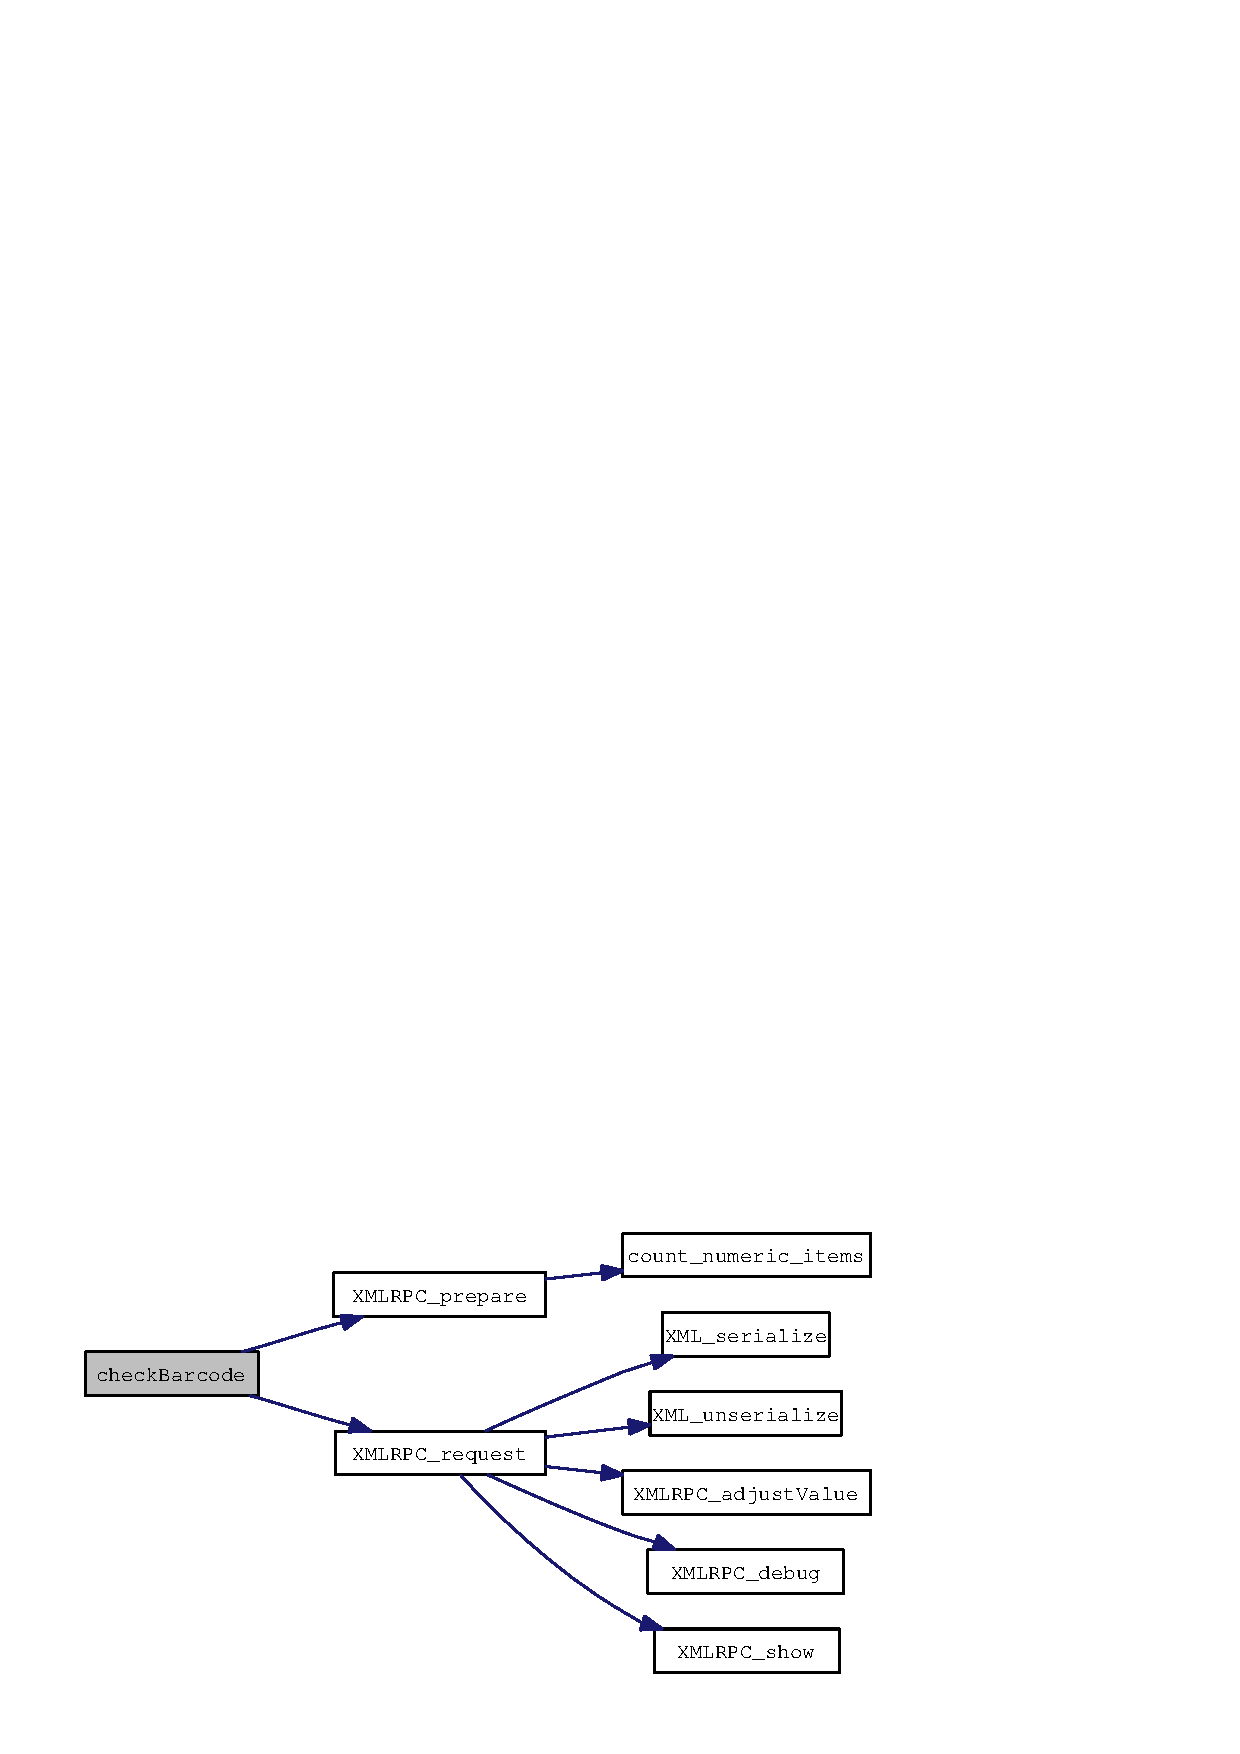
\includegraphics[width=211pt]{barcode_8inc_6d3645af0ef526e4f64d28dcbdceb74f_cgraph}
\end{center}
\end{figure}
\hypertarget{barcode_8inc_e10c37e4f9f9b7c6617a388351a27c99}{
\index{barcode.inc@{barcode.inc}!getBarcodeInfo@{getBarcodeInfo}}
\index{getBarcodeInfo@{getBarcodeInfo}!barcode.inc@{barcode.inc}}
\subsubsection{\setlength{\rightskip}{0pt plus 5cm}getBarcodeInfo (\$ {\em barcode})}}
\label{barcode_8inc_e10c37e4f9f9b7c6617a388351a27c99}


Output Barcode Info \begin{Desc}
\item[Parameters:]
\begin{description}
\item[{\em \$barcode}]The barcode to lookup \end{description}
\end{Desc}
\begin{Desc}
\item[Returns:]HTML code to create the info area \end{Desc}
\begin{Desc}
\item[See also:]\hyperlink{barcode_8inc_6d3645af0ef526e4f64d28dcbdceb74f}{checkBarcode} \end{Desc}


Definition at line 59 of file barcode.inc.

References getImages(), parseXML(), XMLRPC\_\-prepare(), and XMLRPC\_\-request().

\begin{Code}\begin{verbatim}59                                   {
60   switch ($_GET['type']) {
61     case 'upc':
65       $output = '';
66       $output .= '<div id="upc">';
67       $output .= '<img src="upcimg.php?upc=' . $barcode . '" />';
68       $output .= '</div>';
69 
73       $result = XMLRPC_request('dev.upcdatabase.com', '/rpc', 'lookupUPC', array(XMLRPC_prepare($barcode)));
74 //       if ($debug) var_dump($result);
75       echo getImages($result[1]['description']);
76       if ($result[1]['found']) {
77         extract($result[1], EXTR_PREFIX_ALL, 'barcode');
78         $output .= <<<_HTML
79         <div id="info">
80           <table align="center">
81             <tr>
82               <td class="title">Country</td>
83               <td>$barcode_issuerCountry</td>
84             </tr>
85             <tr>
86               <td class="title">Description</td>
87               <td>$barcode_description</td>
88             </tr>
89             <tr>
90               <td class="title">Size</td>
91               <td>$barcode_size</td>
92             </tr>
93           </table>
94           <a href="http://www.upcdatabase.com/editform.asp?upc=$barcode">Modify this entry</a>
95           <a href="http://www.upcdatabase.com/deleteform.asp?upc=$barcode">Delete this entry</a>
96         </div>
97 _HTML;
98       }
99       else {
100         $output .= 'Product Not Found!<br />';
101         $output .= '<a href="http://www.upcdatabase.com/addform.asp?upc=' . $barcode . '">Add this item to the database</a>';
102       }
103       break;
104     case 'isbn':
108       $xml = parseXML('http://isbndb.com/api/books.xml?access_key=' . ISBNKEY . '&index1=isbn&results=texts&value1=' . $barcode);
109 //       var_dump($xml);
110 
111       // Sometimes, the long title is non-existant, so fall back onto the short title
112       if (strlen($xml->BookList->BookData->TitleLong) != 0) {
116         $title = $xml->BookList->BookData->TitleLong;
117       }
118       else {
122         $title = $xml->BookList->BookData->Title;
123       }
127       $author = $xml->BookList->BookData->AuthorsText;
131       $publisher = $xml->BookList->BookData->PublisherText;
135       $summary = $xml->BookList->BookData->Summary;
136 
140       $output = '';
141       $output .= '<div id="upc">';
142       $output .= '<img src="upcimg.php?upc=' . $barcode . '" />';
143       $output .= '</div>';
144       $output .= <<<_HTML
145       <div id="info">
146         <table align="center">
147           <tr>
148             <td class="title">Title</td>
149             <td>$title</td>
150           </tr>
151           <tr>
152             <td class="title">Author</td>
153             <td>$author</td>
154           </tr>
155           <tr>
156             <td class="title">Publisher</td>
157             <td>$publisher</td>
158           </tr>
159           <tr>
160             <td colspan="2">$summary</td>
161           </tr>
162           <tr>
163             <td class="title">Buy</td>
164             <td>
165               <a href="http://www.amazon.com/exec/obidos/ASIN/$barcode/">Amazon.com</a><br />
166               <a href="http://search.barnesandnoble.com/booksearch/isbninquiry.asp?ean=$barcode">Barnes & Noble</a><br />
167               <a href="http://www.booksamillion.com/ncom/books?type=isbn&find=$barcode">Books-A-Million</a><br />
168               <a href="http://www.google.com/products?q=$barcode">Google Product Search</a>
169             </td>
170           </tr>
171         </table>
172       </div>
173 _HTML;
174       break;
175   }
176 
177   return $output;
178 }\end{verbatim}
\end{Code}




Here is the call graph for this function:\nopagebreak
\begin{figure}[H]
\begin{center}
\leavevmode
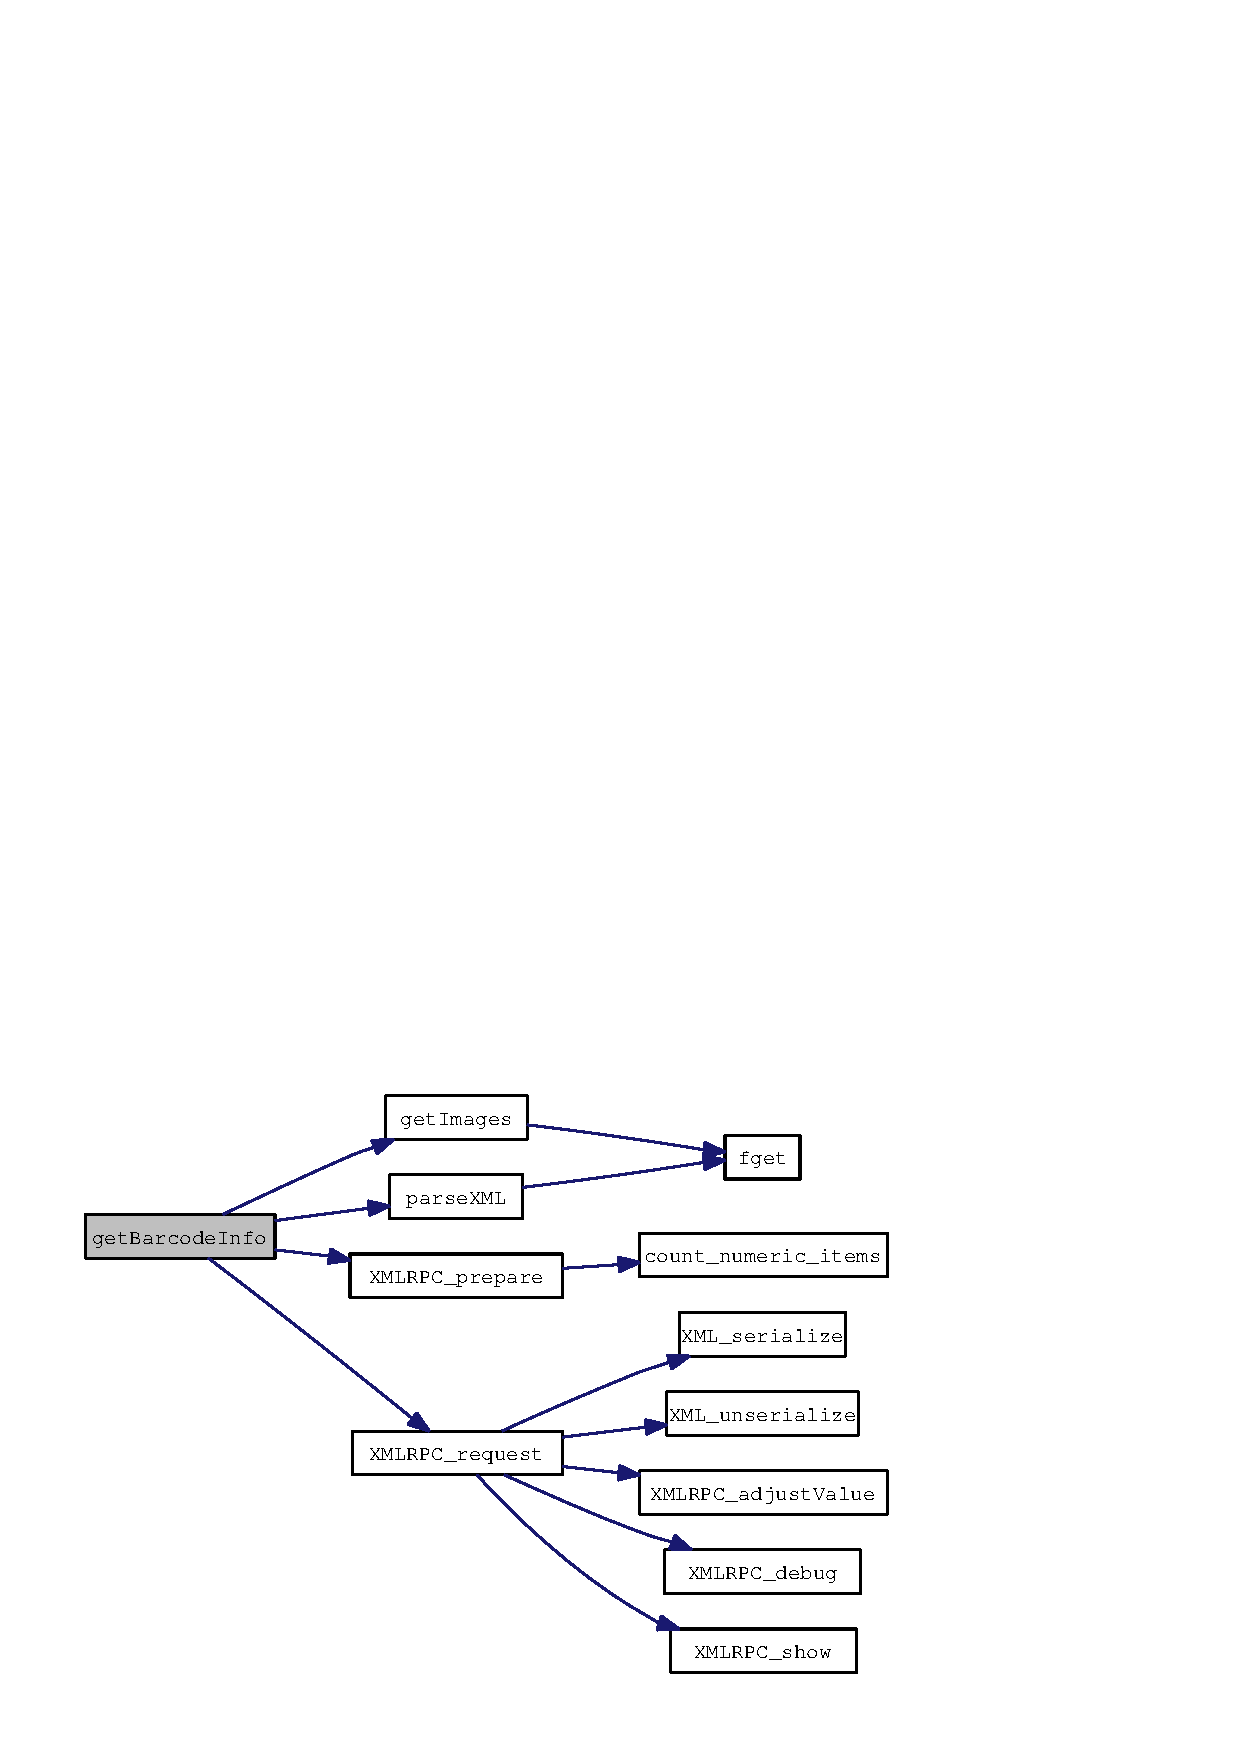
\includegraphics[width=215pt]{barcode_8inc_e10c37e4f9f9b7c6617a388351a27c99_cgraph}
\end{center}
\end{figure}
